%%%%%%%%%%%%%%%%%%%%%%%%%%%%%%%%%%%%%%%%%
% Short Sectioned Assignment LaTeX Template Version 1.0 (5/5/12)
% This template has been downloaded from: http://www.LaTeXTemplates.com
% Original author:  Frits Wenneker (http://www.howtotex.com)
% License: CC BY-NC-SA 3.0 (http://creativecommons.org/licenses/by-nc-sa/3.0/)
%%%%%%%%%%%%%%%%%%%%%%%%%%%%%%%%%%%%%%%%%

%----------------------------------------------------------------------------------------
%	PACKAGES AND OTHER DOCUMENT CONFIGURATIONS
%----------------------------------------------------------------------------------------

\documentclass[paper=a4, fontsize=11pt]{scrartcl} % A4 paper and 11pt font size

% ---- Entrada y salida de texto -----


\usepackage[dvipsnames]{xcolor}
\usepackage{colortbl}
\usepackage{verbatim}
\usepackage{booktabs}
\usepackage{enumitem}
\newlist{subquestion}{enumerate}{1}
\setlist[subquestion,1]{label=(\alph*)}
\usepackage[T1]{fontenc} % Use 8-bit encoding that has 256 glyphs
\usepackage[utf8]{inputenc}
%\usepackage{fourier} % Use the Adobe Utopia font for the document - comment this line to return to the LaTeX default

% ---- Idioma --------

\usepackage[spanish, es-tabla]{babel} % Selecciona el español para palabras introducidas automáticamente, p.ej. "septiembre" en la fecha y especifica que se use la palabra Tabla en vez de Cuadro

% ---- Otros paquetes ----

\usepackage{url} % ,href} %para incluir URLs e hipervínculos dentro del texto (aunque hay que instalar href)
\usepackage{amsmath,amsfonts,amsthm} % Math packages
%\usepackage{graphics,graphicx, floatrow} %para incluir imágenes y notas en las imágenes
\usepackage{graphics,graphicx, float, subfig} %para incluir imágenes y colocarlas

% Para hacer tablas comlejas
%\usepackage{multirow}
%\usepackage{threeparttable}

%\usepackage{sectsty} % Allows customizing section commands
%\allsectionsfont{\centering \normalfont\scshape} % Make all sections centered, the default font and small caps

\usepackage{fancyhdr} % Custom headers and footers
\pagestyle{fancyplain} % Makes all pages in the document conform to the custom headers and footers
\usepackage{eurosym} % Para poder añadir el símbolo del euro
\fancyhead{} % No page header - if you want one, create it in the same way as the footers below
\fancyfoot[L]{} % Empty left footer
\fancyfoot[C]{} % Empty center footer
\fancyfoot[R]{\thepage} % Page numbering for right footer
\renewcommand{\headrulewidth}{0pt} % Remove header underlines
\renewcommand{\footrulewidth}{0pt} % Remove footer underlines
\setlength{\headheight}{13.6pt} % Customize the height of the header

\numberwithin{equation}{section} % Number equations within sections (i.e. 1.1, 1.2, 2.1, 2.2 instead of 1, 2, 3, 4)
\numberwithin{figure}{section} % Number figures within sections (i.e. 1.1, 1.2, 2.1, 2.2 instead of 1, 2, 3, 4)
\numberwithin{table}{section} % Number tables within sections (i.e. 1.1, 1.2, 2.1, 2.2 instead of 1, 2, 3, 4)

\setlength\parindent{0pt} % Removes all indentation from paragraphs - comment this line for an assignment with lots of text

\newcommand{\horrule}[1]{\rule{\linewidth}{#1}} % Create horizontal rule command with 1 argument of height


\usepackage{algpseudocode}
\usepackage[spanish]{babel}
\usepackage{varwidth}
\usepackage{hyperref}
\usepackage{graphicx}
\usepackage{epstopdf}


\selectlanguage{spanish} 
\usepackage[spanish,onelanguage]{algorithm2e} %for psuedo code
\usepackage[lmargin=3.81cm,tmargin=2.54cm,rmargin=2.54cm,bmargin=2.52cm]{geometry}
%\usepackage{listings}
%\usepackage{dsfont}
\usepackage{movie15}
%----------------------------------------------------------------------------------------
%	TÍTULO Y DATOS DEL ALUMNO
%----------------------------------------------------------------------------------------

\title{	
\normalfont \normalsize 
\textsc{\textbf{Metaheurísticas(2019-2020)} \\ Doble Grado en Ingeniería Informática y Matemáticas \\ Universidad de Granada} \\ [25pt] % Your university, school and/or department name(s)
\horrule{0.5pt} \\[0.4cm] % Thin top horizontal rule
\huge Propuesta de metaheurística personalizada \\ para el Problema de la Máxima Diversidad  (MDP) \\ % The assignment title
\horrule{2pt} \\[0.5cm] % Thick bottom horizontal rule
}
\usepackage{movie15}
\author{Alberto Jesús Durán López \\ 
DNI: 54142189-M \\
albduranlopez@gmail.com \\
\hfill \break \hspace{1cm}\\
Grupo Jueves, 17:30 - 19:30 } % Nombre y apellidos


\date{\normalsize\today} % Incluye la fecha actual

%----------------------------------------------------------------------------------------
% DOCUMENTO
%----------------------------------------------------------------------------------------

\begin{document}

\maketitle % Muestra el Título

\newpage %inserta un salto de página

\tableofcontents % para generar el índice de contenidos

% \listoffigures

% \listoftables

\newpage


\section{Introducción}
\hspace{1.5cm} Durante el transcurso de la asignatura se ha trabajado con el problema de la máxima diversidad \textit{(Max Diversity Problem)}. 


En particular, en esta práctica estudiaremos técnicas de búsqueda basadas en poblaciones para la resolución del problema en cuestión. \\
Comentaremos todos los pasos y problemas encontrados, detallando minuciosamente todos los detalles y soluciones a los mismos. \\

Además, se incorporarán tablas para mostrar los resultados de todas las ejecuciones y  gráficas para contrastar los modelos (optimización, costes y desviación).


\section{Problema de la máxima Diversidad}
\hspace{1.5cm} El problema de la máxima diversidad (\textit{maximum diversity problem}, MDP) es un problema de optimización combinatoria consistente en seleccionar un subconjunto de m elementos ($|M|=m$) de un conjunto inicial N de n elementos (con $n>m$) de forma que se maximice la diversidad entre los elementos escogidos. \\


El \textbf{MDP} se puede formular como: \\


\[
\text{Maximizar:   }  z_{MS}(x) = \sum_{i=1}^{n-1} \sum_{j=i+1}^{n} d_{ij}x_i x_j
\]



\[
\text{Sujeto a: } \sum_{i=1}^{n} x_i=m \hspace{0.2cm} \text{ con } x_i=\{0,1\} \text{, } i=1,...,n  \hspace{0.5cm} \text{donde: }
\]


\begin{itemize}
	\item x es una solución al problema que consiste en un vector binario que indica los m elementos seleccionados.
	\item $d_{ij}$ es la distancia existente entre los elementos $i$ y $j$
	
\end{itemize}


\begin{figure}[H]
	\centering
	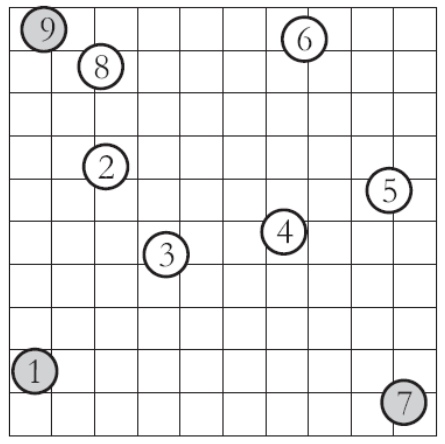
\includegraphics[scale=0.35]{img/mdp.png}
	\caption{MDP-Maximum Diversity Problem}
\end{figure}


\newpage
\subsection{Datos y casos considerados}
\hspace{1.5cm} Las ejecuciones se han realizado en un ordenador \texttt{Intel(R) Core(TM) i7-1065G7 CPU @ 1.30GHz, 16GB RAM, 512 SSD}. 


Se utilizarán \textbf{30 casos} seleccionados de varios de los conjuntos de instancias disponible en la \href{http://www.optsicom.es/mdp/}{MDPLIB}, 10 pertenecientes al grupo \texttt{GKD} con distancias Euclideas, n=500 y m=50 \textit{(GKD-c\_11\_n500\_m50 a GKD-
c\_20\_n500\_m50)}, 10 del grupo \texttt{MDG} con distancias reales en [0,1000], n=500 y m=50
\textit{(MDG-b\_1\_n500\_m50 a MDG-b\_10\_n500\_m50)}; y otras 10 del grupo \texttt{MDG} con distancias enteras en {0,10}, n=2000 y m=200 \textit{(MDG-a\_31\_n2000\_m200 a MDG-
a\_40\_n2000\_m200)}. \\


Para la realización de la práctica usaremos el lenguaje de programación \texttt{C++} ya que se deben probar muchos ejemplos y la ejecución es más rápida al ser un lenguaje de programación compilado. \\
Todos los archivos se han compilado con la opción de optimización \texttt{-O2} y, además,  la semilla usada para todas
las ejecuciones ha sido 54142189, pudiéndose ésta indicar en la ejecución del archivo en cuestión. 







\subsection{Descripción de la Función Objetivo}

Todos los algoritmos implementados hacen uso de la misma función objetivo, la comentada en el punto (2) anterior y cuyo pseudocódigo mostramos a continuación. Bien es cierto que en el caso de la \textit{Búsqueda Local} se tiene que usar codificación basada en números enteros, sin embargo, dicha función se ve mínimamente modificada.


\begin{figure}[H]
	\centering
	\begin{minipage}{.9\linewidth}
		
		
		
		\begin{algorithm}[H] 
			

			\SetAlgoLined
			
			\KwData{\textbf{ContribucionIndep}(\textit{integer ind, vector sel, matriz distancias)}}
			
			\Begin{
				\textit{suma $\leftarrow$ 0} \;
				
				\For{j in sel}{
					$ suma \leftarrow sel[j]\cdot(distancias[ind][j] + suma)$ \;	
				}
				
				\Return $suma$
			}
			
		\end{algorithm} 
		
	\end{minipage}
\end{figure}



\begin{figure}[H]
	\centering
	\begin{minipage}{.9\linewidth}
		
		
		
		\begin{algorithm}[H] 
			
			\caption{Evaluar solución}
			\SetAlgoLined
			
			\KwData{\textbf{CosteEstimado}(\textit{vector sel, matriz distancias)}}
			
			\Begin{
				
				\textit{suma $\leftarrow$ 0} \;
				
				
				\For{i in $|sel|$}{
					\If{$sel[i]=true$}{
						$ suma \leftarrow ContribucionIndep(i, sel, distancias) + suma$ \;
					}
					
				}
				
				\Return $suma/2$
			}
			
		\end{algorithm} 
		
	\end{minipage}
\end{figure}


\newpage 
\section{Metaheurística original propuesta}

Los juegos clásicos que todos conocemos como el buscaminas, tetris o pacman, entre otros, se caracterizan por hacer uso de un tablero o, mejor dicho, un plano finito para su representación.

Esto quiere decir que estos juegos funcionan en un recinto acotado, no pudiendo las diferentes componentes del juego salir de éste. \\

Por otro lado, existen otros juegos como el \textit{snake} que hacen uso de un tablero cuya superficie es un toro llano. En ésta, cuando la serpiente sale por arriba, entra por abajo y al igual ocurre con los lados, si sale por la derecha, entrará por la izquierda y viceversa.

Es decir, podemos establecer una identificación con los bordes de forma que aplicando transformaciones topológicas podemos obtener un toroide tal y como se muestra en la siguiente imagen:

\begin{figure}[H]
	\centering
	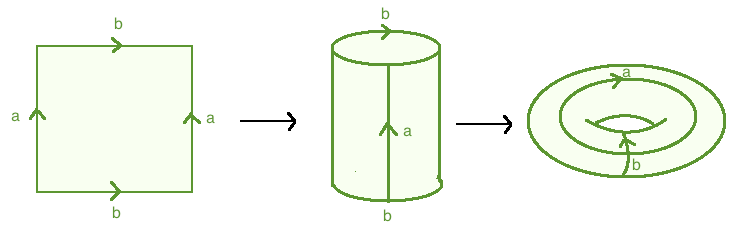
\includegraphics[scale=0.35]{img/toro.png}
	\caption{Pegado de un toro}
	\label{toro}
\end{figure}

Puede además dirigirse al siguiente \href{https://www.youtube.com/watch?v=0KwGE6hAtGc}{enlace} para ver de forma animada como se lleva a cabo este pegado. \\

Como podemos imaginar, el toro llano o toroide no es la única superficie que se puede construir identificando lados. De hecho, estas superficies admiten una clasificación que comentamos a continuación:


\begin{itemize}
	\item  Una superficie es \textbf{no orientable} si existe al menos una curva cerrada simple contenida que es homeomorfa a una banda de Möbius. Ejemplos: 
	
	\begin{enumerate}
		\item \texttt{Banda de Möbius}: \href{https://www.youtube.com/watch?v=fCJ0mCUaEok}{pegado}
				\begin{figure}[H]
				\centering
				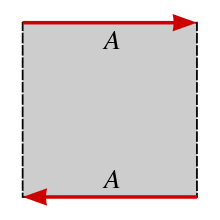
\includegraphics[scale=0.3]{img/idb.png}
				\qquad
				
\includegraphics[scale=0.25]{img/flecha.png}
				\qquad
				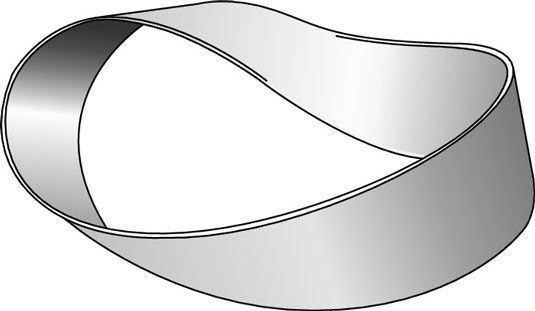
\includegraphics[scale=0.3]{img/banda.png}
				
				\caption{Pegado de una banda de Möbius}
			\end{figure}
		
		\item \texttt{Plano Proyectivo}: Quizás las siguientes superficies necesiten algo más de visión espacial ya que el \href{https://www.youtube.com/watch?v=W-sKLN0VBkk}{pegado} no es tan trivial.
		\begin{figure}[H]
			\centering
			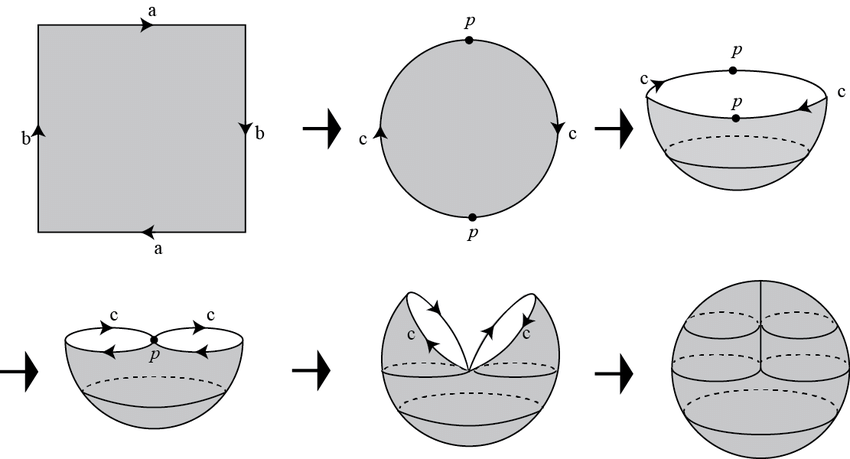
\includegraphics[scale=0.35]{img/a.png}
			\caption{Pegado de un Plano Proyectivo}
		\end{figure}
		
		\item \texttt{Botella de Klein}: \href{https://www.youtube.com/watch?v=yaeyNjUPVqs}{Enlace}
		
					\begin{figure}[H]
				\centering
				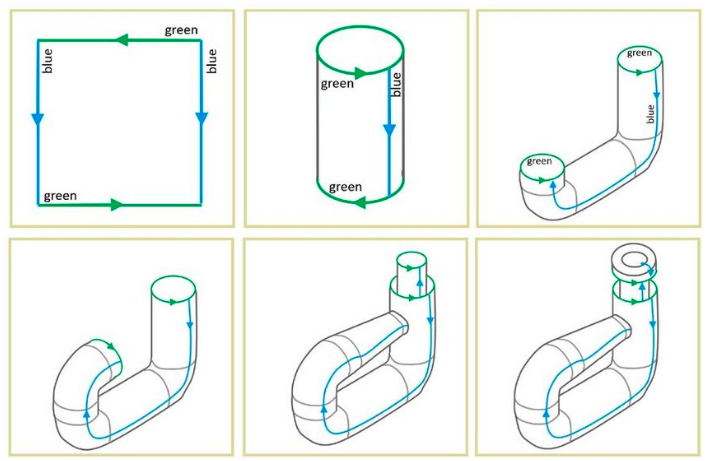
\includegraphics[scale=0.4]{img/klein.png}
				\caption{Pegado de una Botella de Klein}
			\end{figure}
	\end{enumerate}
	

	\item En caso contrario, la superficie será \textbf{orientable}. Ejemplos: Toro llano \ref{toro}, cilindro, suma conexa de k-toros...etc
\end{itemize}

\subsection{Adaptación de la propuesta al problema MDP}


Recordando nuestro problema MDP, teníamos que escoger un subconjunto de m elementos de un conjunto inicial de \textbf{n} elementos de forma que se maximice la diversidad entre los elementos escogidos. A este conjunto se le suele denominar \textit{sel} (seleccionados) y en una primera versión implementada está creado de forma aleatoria.

En la sección anterior hemos visto como a partir de identificaciones en los bordes de un cuadrado podemos dar lugar a diferentes superficies, por ello, he tomado diferentes soluciones (generadas aleatoriamente) que viven en cada una de las superficies para ver cómo se comportan.


Las características que rigen el comportamiento de nuestro algoritmo son las siguientes:

\begin{itemize}
	\item \texttt{Movimiento}: La operación que simula cada identificación será una mutación. ¿Cómo haremos esto? Relacionándolos de forma que identificaciones en el mismo sentido serán mutaciones en el mismo caracter/posición, mientras que mutaciones en sentidos opuestos serán mutaciones en las posiciones $k$ y $n-k$, respectivamente. (n es el tamaño de la población).
	
	
	\begin{figure}[H]
		\centering
		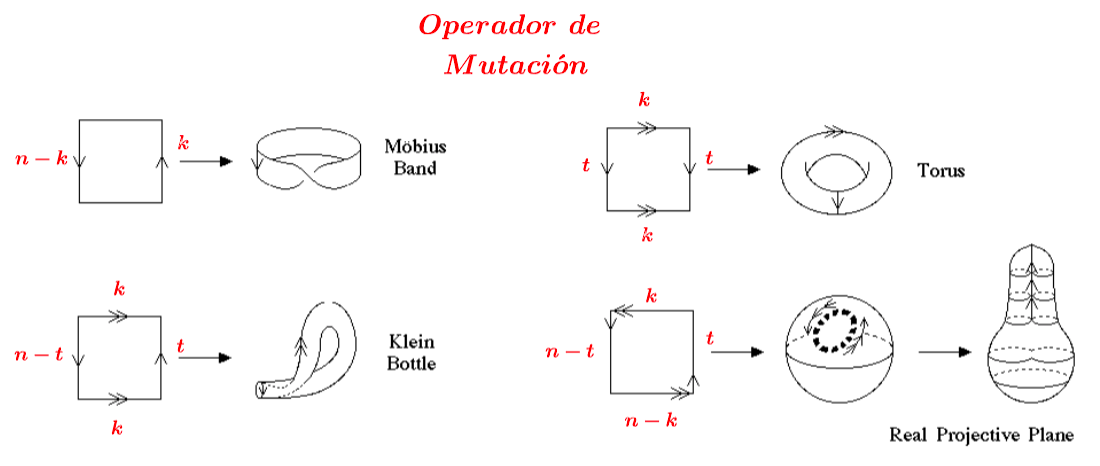
\includegraphics[scale=0.38]{img/topo6.png}
	\end{figure}
	
	
		A modo de ejemplo, lo explicaremos con el famoso juego del \textit{Snake} en la superficie de Toro llano cuyo modelo es el que ha seguido nuestra implementación.
		
	Cuando nuestra serpiente sale por la parte superior, se muta el carácter $k$, igual que si sale por la parte inferior, ya que en un toro las partes superior e inferior están identificadas. Cuando la serpiente sale por la izquierda o derecha, se muta otro caracter $t$, ya que ambos lados también están identificados pero son distintos al anterior.
	
	Con esto conseguimos entornos amplios y variados, cada uno caracterizado por tener una exploración de una región distinta. \\
	
	
	\item \texttt{Nutrición}: Siguiendo con las reglas del \textit{Snake}, en todo momento hay un pixel en el tablero que hace referencia a 'comida' que nuestra serpiente puede coger para crecer. En nuestro programa se simulará lo mismo haciendo uso de una distribución uniforme en el intervalo [0,1]. Cuando cada serpiente haya obtenido un número de alimento igual a $\frac{n}{3}$, nuestra solución será lo suficientemente capaz para tener descendencia y dar lugar a una nueva solución en la que se ha producido una mutación brusca (para dar lugar a hijos diferentes en gran medida a los padres y así evitar óptimos locales). 
	
	Los valores de la Distribución Uniforme se han elegido de acuerdo a numerosas pruebas para que las soluciones no crezcan en exceso (ya que a mayor número de soluciones se gastan más evaluaciones de la función objetivo produciendo así una menor convergencia). 
	

	

	
	
\end{itemize}

\newpage 
\subsection{Mejoras tenidas en cuenta en esta primera versión}
\begin{enumerate}
	\item \texttt{Mejora en la representación}: Para todos los algoritmos menos para la \textit{Búsqueda Local}, se ha usado una codificación basada en números binarios. Sin embargo, dejaremos la explicación para las siguientes secciones, donde se explicará con detalle en cada algoritmo.
	
	En relación con la estructura de datos usada, tras varias pruebas se ha optado por la modularización en una clase denominada \textit{Superficie} en la que se le ha de indicar en el constructor los índices referentes a la mutación de cada superficie.
	
	

	
	\item Para favorecer la convergencia se ha tenido en cuenta el factor elitista. En cada superficie, si la mejor solución del estado anterior no sobrevive, sustituye directamente la peor solución del estado siguiente. ¿Por qué únicamente la mejor? Para evitar así la convergencia prematura y explorar el máximo de entornos posibles.
	
	\item \texttt{Modelo Distribuido. Modelo isla para añadir un operador de viaje}: Tenemos soluciones en diferentes superficies que han ido evolucionando en paralelo pero de forma independiente, explorando así distintas regiones del espacio ya que el operador de mutación aplicado es distinto en cada una de ellas. \\
	
	\begin{figure}[H]
		\centering
		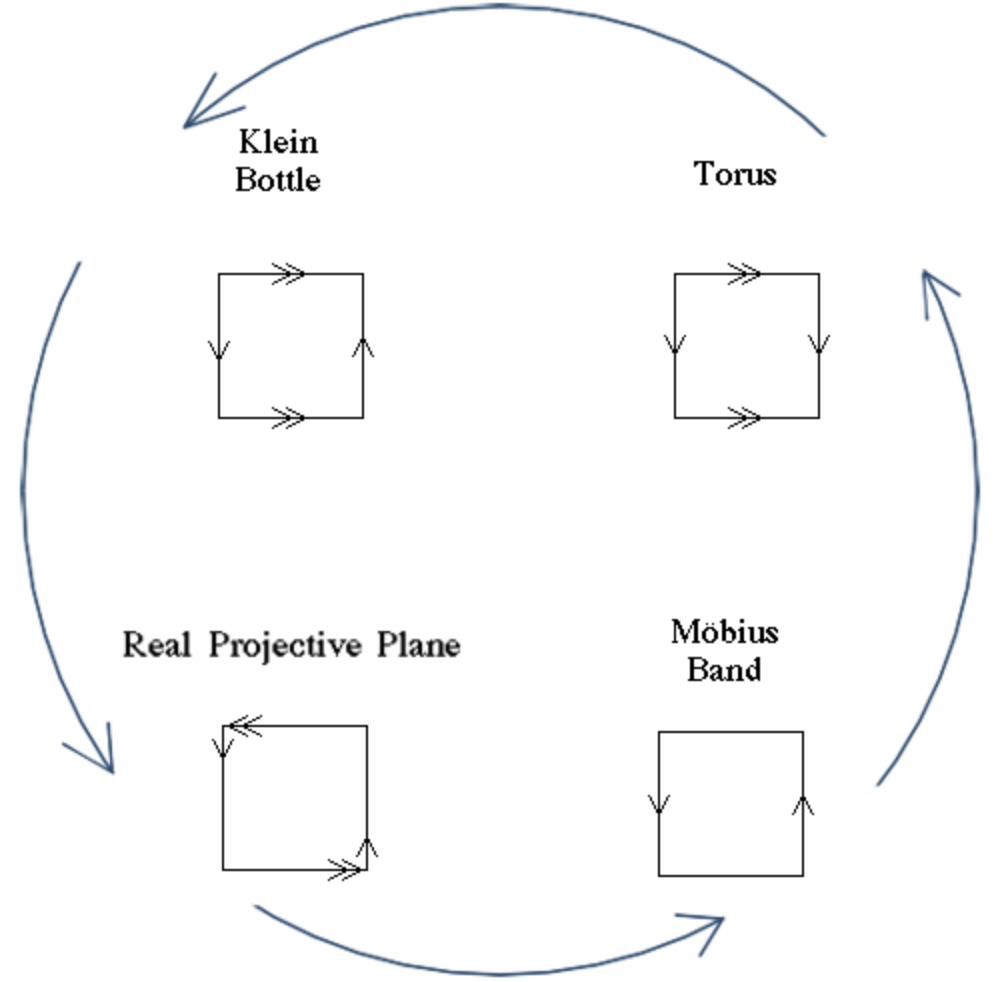
\includegraphics[scale=0.3]{img/perf.png}
		\caption{Modelo Distribuido}
	\end{figure}
	
	
	\begin{itemize}
		\item 	Establecemos un operador de viaje en el que la mejor solución de cada Superficie podrá viajar a otra y seguir con el mismo proceso de crecimiento descrito hasta aquí pero con aplicándole un nuevo operador de mutación.
		
		\item 	Se sigue una estructura de intercomunicación en forma de Anillo ya que el sentido de flujo es único.
		
		\newpage 
		
		\item  En una primera versión implementada la solución pasaba a otra superficie sin copiarse. Sin embargo, los resultados empeoraban ya que la solución era muy buena en el entorno explorado anterior, pero no tanto cuando se aplicaba el operador de mutación de la nueva superficie.
	 Por ello, el viaje consistirá en una copia de la mejor solución de una superficie a otra para que así nuestra mejor solución pueda seguir explorándose en diferentes superficies.
		
		\item 	Este modelo distribuido proporciona una búsqueda más efectiva que la evolución de una gran población en el que todas las soluciones coexistieran.
	\end{itemize}
 
	

	


	
	\item Las soluciones iniciales están formadas aleatoriamente, por ello, a esta aleatoriedad se han añadido soluciones de calidad obtenidas a partir del algoritmo de \textit{Búsqueda Tabú}. Tendremos un 50\% de soluciones obtenidas de forma aleatoria y otro 50\% de soluciones de la \textit{B. Tabú}. Éste, se introducirá en las siguientes secciones y con él, favorecemos el equilibrio \textit{<<Exploración - Explotación>>}
\end{enumerate}


	\begin{figure}[H]
	\centering
	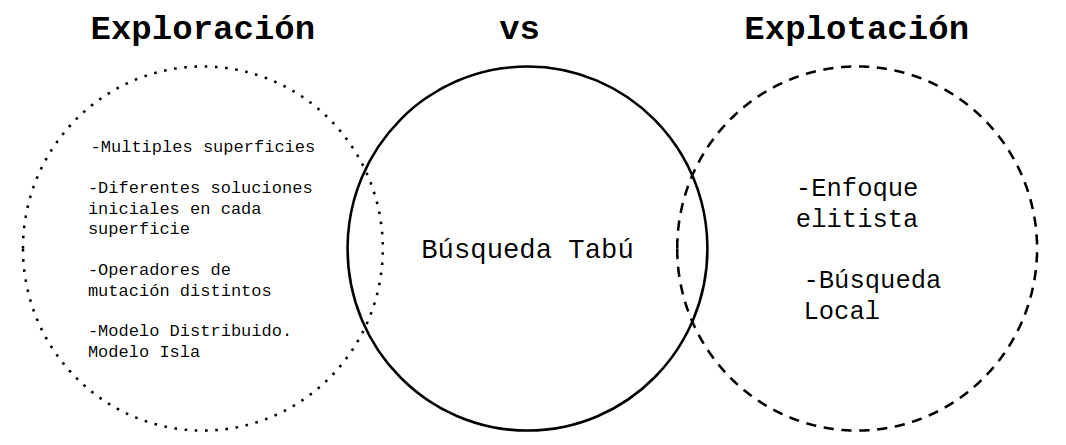
\includegraphics[scale=0.35]{img/lol.png}
	\caption{Mejoras propuestas}
\end{figure}


\newpage 

\section{<<Exploración-Explotación>> Multi-Entorno}

Al tener tantas superficies caracterizadas por tener mutaciones distintas, me ha parecido adecuado llamar a esta propuesta \textit{<<Explotación-Explotación>> Multi-Entorno}.

El pseudocódigo asociado es el que se muestra a continuación y que explicaremos brevemente:

\begin{itemize}
	\item Primeramente, creamos las diferentes superficies \textit{Botella de Klein, Plano proyectivo, Cinta de Möbius y Toro llano}. El constructor de la clase se encargará de asignar mutaciones diferentes a cada una de ellas.
	\item En segundo lugar, las distintas soluciones que habitan en cada superficie se crearán de forma aleatoria llamando a la función \textbf{SolucionAleatoria}.
	\item A continuación, se lleva a cabo el bucle principal en el que cada solución se mueve libremente por la superficie, coge comida (\textit{nutrirse}) y si la solución crece hasta $\frac{n}{2}$ de su tamaño original es capaz de mudar la piel y dar lugar a nuevas soluciones.
	\item Por último, dadas dos superficies, la mejor solución de una de ellas viajará a otra (se copiará), pasando así a modificar el operador de mutación que se le aplica (modelo distribuido-isla)
\end{itemize}



\begin{figure}[H]
	\centering
	\begin{minipage}{.75\linewidth}
		
		\begin{algorithm}[H] 
			\caption{Mundo Superficie }
			\SetAlgoLined
			
			\KwData{\textbf{MundoSuperficie}}
			
			
			\Begin{
				$Superficies \leftarrow $ \{\textit{Botella de Klein, Plano proyectivo,} \hspace*{2.4cm}  \textit{Cinta de Möbius, Toro llano} \} \;
				
				\hfill \break
				\For{$s \in Superficies[i]$, $i = 1,...,|Superficies|$}{
					$s \leftarrow$ \textbf{SolucionAleatoria(n,m)} \;
					
				}
				\While{$eval < n\_eval$}{
					\For{$s \in Superficies[i]$, $i = 1,...,|Superficies|$}{
						$movimiento$ \;
						%$evaluarPoblacion$ \;
						$nutrirse$ \;
						$mudar\_piel$ \;	
					}
				
					\If{\textit{se dan las condiciones para viajar}}{
						\For{$s, s' = Superficies[i], Superficies[i+1]$}{
							%\textit{aplicar\_BL a los} $\frac{n}{2}$ \textit{peores de la población de s} \;
							\textit{s viaja a s'}\;
						}	
					}
				}
			}
		\end{algorithm}
	\end{minipage}
\end{figure}











\newpage 
\section{Búsqueda Local}
\hspace{1.5cm}El algoritmo de \textit{Búsqueda Local} usado para nuestro algoritmo se corresponde con el implementado en la primera práctica, por ello, conviene recordar como funciona: 

\begin{itemize}
	
	
	
	\item Función de intercambio, Int(sel,i,j). El parámetro \texttt{i} indica el índice del elemento que se eliminará de la solución y el j por cual se sustituirá. Por tanto, las opciones para \texttt{i} serán \texttt{m} (los m elementos seleccionados) y las opciones para \texttt{j} serán \texttt{n-m} (los elementos disponibles en \textit{no seleccionados}), por tanto, el entorno estará formado por \texttt{m$\cdot$(n-m)} elementos.
	
	
	
	\begin{figure}[H]
		\centering
		\begin{minipage}{.75\linewidth}
			
			\begin{algorithm}[H] 
				\caption{EvaluaVecinos }
				\SetAlgoLined
				
				\KwData{\textbf{EvaluaVecinos}}
				
				
				\Begin{
					
					$mejora \leftarrow True$\;
					$eval \leftarrow 0$ \;
					
					\break \hfill
					
					
					\While{\textit{eval<100.000 and mejora}}{
						
						
						
						\break \hfill
						
						\hspace{3cm}\textbf{. . .}
						
						
						
						\break \hfill
						
						$salir \leftarrow$ False, $c \leftarrow 0$ \;
						
						\While{$c< n-m$ and not salir}{
							
							\textit{Genera elemento válido j} \;
							
							\If{\texttt{Contrib($s_j$)}>\texttt{Contrib($s_i$)}}{
								
								\textit{Int(sel, i, j)} \;
								$salir \leftarrow$ True\;
								$coste\leftarrow coste + contribNueva - contribAntigua$ 
							}
							$c\leftarrow c+1$\;
							$eval\leftarrow eval+1$\;
						}
					}
				}
			\end{algorithm}
		\end{minipage}
	\end{figure}
	
	
	\item En cada iteración, podemos calcular la diferencia de costes entre las dos soluciones recalculando todas las distancias de la función objetivo, sin embargo, esto no es necesario ya que como únicamente añadimos y quitamos 1 elemento, basta con sumar y restar la distancia del nuevo y del viejo elemento al resto de elementos seleccionados, respectivamente. Además, combinamos la factorización del coste con el cálculo de la contribución de los elementos para mejorar aún más la eficiencia.
	
	
	
	Si el intercambio es favorable, es decir, si el coste de la nueva solución (sumando las distancias del nuevo elemento y restando las del elemento anterior) es mayor que la anterior, aceptamos el intercambio. En caso contrario, rechazamos.
	
	\item Repetiremos este proceso hasta que se realicen \textit{N} evaluaciones de la función objetivo o cuando no encuentre mejora en el entorno.
	
\end{itemize}

\newpage 
\subsection{Hibridación de nuestro problema con Búsqueda Local}
Ahora bien, se explicará la forma de hibridación escogida según los resultados obtenidos en los algoritmos meméticos de la práctica 2.
En estos, había que programar varias versiones, variando entre aplicar Búsqueda Local a toda la población o una parte de ella.

Adicionalmente, se realizó otra versión explorando los $\frac{n}{2}$ peores cromosomas de la población obteniendo incluso mejores resultados que explorar toda la población o una mejor parte de ella.


Por esto, se han realizado pruebas aplicando BL sobre toda la población, mejores soluciones y peores soluciones, obteniendo también mejores resultados aplicando la hibridación sobre los $\frac{n}{2}$ peores soluciones.

El pseudocódigo anterior no se ve modificado a excepción de la siguiente parte:




\begin{figure}[H]
	\centering
	\begin{minipage}{.75\linewidth}
		
		\begin{algorithm}[H] 
			\caption{Hibridación }
			\SetAlgoLined
			
			\KwData{\textbf{MundoSuperficie}}
			
			
			\Begin{
						\break \hfill
					
					\hspace{3cm}\textbf{. . .}
					
					
					\break 
				\If{\textit{se dan las condiciones para viajar}}{
					\For{$s, s' = Superficies[i], Superficies[i+1]$}{
						\textit{aplicar\_BL a los} $\frac{n}{2}$ \textit{peores de la población de s} \;
						\textit{s viaja a s'}\;
					}	
				}
				
			}
		\end{algorithm}
	\end{minipage}
\end{figure}




Parados en este punto, nos preguntamos: ¿qué ventajas nos ofrece aplicar \textit{BL} sobre la peor parte de la población?

	\begin{figure}[H]
	\centering
	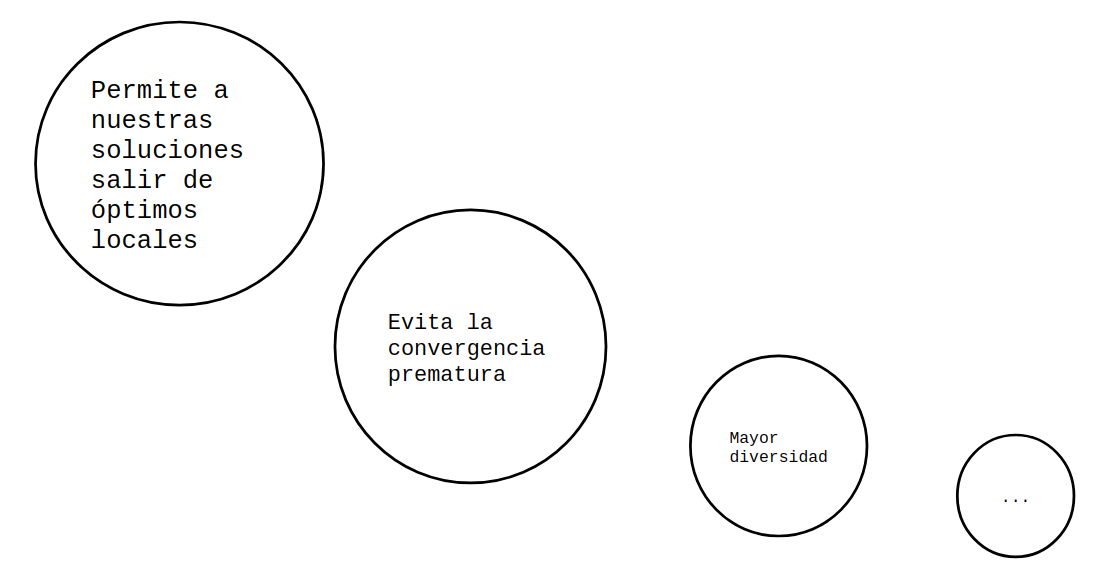
\includegraphics[scale=0.35]{img/def.png}
\end{figure}























\newpage
\section{Búsqueda Tabú}

La \textit{Búsqueda Tabú} es una metaheurística que utiliza un procedimiento de búsqueda heurística local para explorar el espacio de la solución que pertenece a un óptimo local. Uno de los principales características de este método es el uso de memoria adaptativa, que hace que el comportamiento de búsqueda sea más flexible.Se usarán dos listas:
\begin{itemize}
	\item \texttt{freq}: Almacena el número de veces que el elemento $s_i$ ha sido seleccionado en construcciones previas donde $max\_freq$ representa el máximo valor de $freq[i]$ $\forall i \in {0,...,n}$
	
	\item \texttt{quality}: En esta lista se almacena la media de las soluciones previas en las que el elemento $s_i$ ha sido seleccionado. Por otro lado, $max\_q$ hace referencia al máximo valor de $quality[i]$ $\forall i$, $i \in {0,...,n}$
\end{itemize}

El objetivo es el de usar estar dos listas para formar la solución tomando los elementos más atractivos del total de disponibles: 
\begin{itemize}
	\item \textit{S}: Elementos totales, \textit{sel}: seleccionados, \textit{S-sel}: Elementos disponibles pero no seleccionados
	
	\item $s\_center$: devuelve el elemento que se corresponde con el centro de gravedad del conjunto pasado por argumento y $\beta$ y $\delta$ sirven para incidir en el peso de los valores explicados anteriormente.
\end{itemize}
Para ello, en cada iteración se modificará la construcción de la solución evaluando la atractividad de cada elemento de \textit{S-sel}. Esto se llevará a cabo dependiendo de los valores que tomen las listas anteriores, favoreciendo los elementos con bajas frecuencias y alta calidad. 

Mostramos a continuación el pseudocódigo asociado a la función principal del algoritmo:

\begin{figure}[H]
	\centering
	\begin{minipage}{.895\linewidth}
		
		
		
		\begin{algorithm}[H] 
			
			\caption{Búsqueda Tabú}
			\SetAlgoLined
			
			\KwData{\textbf{BusquedaTabu}}
			
			\Begin{
				
				
				$freq[i] = quality[i] = 0 $ $\forall s_i \in S$ \;
				
				
				\For{$eval < n\_eval$}{
					$sel \leftarrow \emptyset$ \;
					$s_c = s\_center(S)$ \;
					\While{$|sel|<m$}{
						\For{$s_i \in S-sel$}{
							$d'(s_i,s_c) \leftarrow d(s_i,s_c)-\beta d(s_i,s_c)\frac{freq[i]}{max\_freq}+\delta d(s_i,s_c)\frac{quality[i]}{max\_q}$ \;
						}
						\textit{Tomar $i^*$ tal que} $d'(s_{i^*},s_c)=max\{d'(s_i,s_c)\}$ \;
						$freq[i^*] \leftarrow freq[i^*]+1 $\;
						$sel \leftarrow sel \cup s_{i^*}$ \;
						$S \leftarrow S-s_{i^*}$\;
						$s_c \leftarrow s\_center(sel)$\;
					}
					$z \leftarrow Coste$$Solucion(sel)$ \;
					
					\For{$s_i \in sel$}{
							$quality[i] \leftarrow \frac{quality[i](freq[i]-1)+z}{freq[i]}$ \;
					}
				}
				
			}
			
		\end{algorithm} 
		
	\end{minipage}
\end{figure}

\newpage











\section{Resultados Obtenidos}


% Please add the following required packages to your document preamble:
% \usepackage{booktabs}
% \usepackage{graphicx}
% \usepackage[table,xcdraw]{xcolor}
% If you use beamer only pass "xcolor=table" option, i.e. \documentclass[xcolor=table]{beamer}
\begin{table}[H]
	\centering
	\resizebox{\textwidth}{!}{%
		\begin{tabular}{@{}
				>{\columncolor[HTML]{FFFFFF}}c 
				>{\columncolor[HTML]{FFFFFF}}c 
				>{\columncolor[HTML]{FFFFFF}}c 
				>{\columncolor[HTML]{FFFFFF}}c 
				>{\columncolor[HTML]{FFFFFF}}c 
				>{\columncolor[HTML]{FFFFFF}}c 
				>{\columncolor[HTML]{FFFFFF}}c 
				>{\columncolor[HTML]{FFFFFF}}c @{}}
			\toprule
			{\color[HTML]{000000} \textbf{Instancia}}     & {\color[HTML]{000000} \textbf{\begin{tabular}[c]{@{}c@{}}Mejor \\ Coste\end{tabular}}} & {\color[HTML]{000000} \textbf{Superficies}} & {\color[HTML]{000000} \textbf{Desv}} & \textbf{\begin{tabular}[c]{@{}c@{}}Superf.\\ + BL\end{tabular}} & \textbf{Desv}               & \textbf{\begin{tabular}[c]{@{}c@{}}Superficies\\ BTabú+BL\end{tabular}} & \textbf{Desv}               \\ \midrule
			{\color[HTML]{000000} GKD-c\_11\_n500\_m50}   & {\color[HTML]{000000} 19587,13}                                                        & {\color[HTML]{000000} 19567,2}              & {\color[HTML]{000000} 0,10}          & {\color[HTML]{000000} 19585,7}                                  & {\color[HTML]{000000} 0,01} & {\color[HTML]{000000} 19585,80}                                         & {\color[HTML]{000000} 0,01} \\
			{\color[HTML]{000000} GKD-c\_12\_n500\_m50}   & {\color[HTML]{000000} 19360,24}                                                        & {\color[HTML]{000000} 19333,9}              & {\color[HTML]{000000} 0,14}          & {\color[HTML]{000000} 19360,2}                                  & {\color[HTML]{000000} 0,00} & {\color[HTML]{000000} 19359,70}                                         & {\color[HTML]{000000} 0,00} \\
			{\color[HTML]{000000} GKD-c\_13\_n500\_m50}   & {\color[HTML]{000000} 19366,7}                                                         & {\color[HTML]{000000} 19327,8}              & {\color[HTML]{000000} 0,20}          & {\color[HTML]{000000} 19366,7}                                  & {\color[HTML]{000000} 0,00} & {\color[HTML]{000000} 19357,80}                                         & {\color[HTML]{000000} 0,05} \\
			{\color[HTML]{000000} GKD-c\_14\_n500\_m50}   & {\color[HTML]{000000} 19458,56}                                                        & {\color[HTML]{000000} 19443,3}              & {\color[HTML]{000000} 0,08}          & {\color[HTML]{000000} 19458,6}                                  & {\color[HTML]{000000} 0,00} & {\color[HTML]{000000} 19458,60}                                         & {\color[HTML]{000000} 0,00} \\
			{\color[HTML]{000000} GKD-c\_15\_n500\_m50}   & {\color[HTML]{000000} 19422,15}                                                        & {\color[HTML]{000000} 19381,5}              & {\color[HTML]{000000} 0,21}          & {\color[HTML]{000000} 19422,1}                                  & {\color[HTML]{000000} 0,00} & {\color[HTML]{000000} 19413,10}                                         & {\color[HTML]{000000} 0,05} \\
			{\color[HTML]{000000} GKD-c\_16\_n500\_m50}   & {\color[HTML]{000000} 19680,21}                                                        & {\color[HTML]{000000} 19638,2}              & {\color[HTML]{000000} 0,21}          & {\color[HTML]{000000} 19680,2}                                  & {\color[HTML]{000000} 0,00} & {\color[HTML]{000000} 19670,40}                                         & {\color[HTML]{000000} 0,05} \\
			{\color[HTML]{000000} GKD-c\_17\_n500\_m50}   & {\color[HTML]{000000} 19331,39}                                                        & {\color[HTML]{000000} 19285,4}              & {\color[HTML]{000000} 0,24}          & {\color[HTML]{000000} 19331,4}                                  & {\color[HTML]{000000} 0,00} & {\color[HTML]{000000} 19322,30}                                         & {\color[HTML]{000000} 0,05} \\
			{\color[HTML]{000000} GKD-c\_18\_n500\_m50}   & {\color[HTML]{000000} 19461,39}                                                        & {\color[HTML]{000000} 19405,3}              & {\color[HTML]{000000} 0,29}          & {\color[HTML]{000000} 19461,4}                                  & {\color[HTML]{000000} 0,00} & {\color[HTML]{000000} 19446,70}                                         & {\color[HTML]{000000} 0,08} \\
			{\color[HTML]{000000} GKD-c\_19\_n500\_m50}   & {\color[HTML]{000000} 19477,39}                                                        & {\color[HTML]{000000} 19435,1}              & {\color[HTML]{000000} 0,22}          & {\color[HTML]{000000} 19477,3}                                  & {\color[HTML]{000000} 0,00} & {\color[HTML]{000000} 19473,50}                                         & {\color[HTML]{000000} 0,02} \\
			{\color[HTML]{000000} GKD-c\_20\_n500\_m50}   & {\color[HTML]{000000} 19604,84}                                                        & {\color[HTML]{000000} 19585,6}              & {\color[HTML]{000000} 0,10}          & {\color[HTML]{000000} 19604,8}                                  & {\color[HTML]{000000} 0,00} & {\color[HTML]{000000} 19601,80}                                         & {\color[HTML]{000000} 0,02} \\
			{\color[HTML]{000000} MDG-b\_1\_n500\_m50}    & {\color[HTML]{000000} 778030,62}                                                       & {\color[HTML]{000000} 752733}               & {\color[HTML]{000000} 3,25}          & {\color[HTML]{000000} 769661}                                   & {\color[HTML]{000000} 1,08} & {\color[HTML]{000000} 771034}                                           & {\color[HTML]{000000} 0,90} \\
			{\color[HTML]{000000} MDG-b\_2\_n500\_m50}    & {\color[HTML]{000000} 779963,69}                                                       & {\color[HTML]{000000} 763458}               & {\color[HTML]{000000} 2,12}          & {\color[HTML]{000000} 768273}                                   & {\color[HTML]{000000} 1,50} & {\color[HTML]{000000} 774127}                                           & {\color[HTML]{000000} 0,75} \\
			{\color[HTML]{000000} MDG-b\_3\_n500\_m50}    & {\color[HTML]{000000} 776768,44}                                                       & {\color[HTML]{000000} 757101}               & {\color[HTML]{000000} 2,53}          & {\color[HTML]{000000} 767690}                                   & {\color[HTML]{000000} 1,17} & {\color[HTML]{000000} 767466}                                           & {\color[HTML]{000000} 1,20} \\
			{\color[HTML]{000000} MDG-b\_4\_n500\_m50}    & {\color[HTML]{000000} 775394,62}                                                       & {\color[HTML]{000000} 748318}               & {\color[HTML]{000000} 3,49}          & {\color[HTML]{000000} 763243}                                   & {\color[HTML]{000000} 1,57} & {\color[HTML]{000000} 767486}                                           & {\color[HTML]{000000} 1,02} \\
			{\color[HTML]{000000} MDG-b\_5\_n500\_m50}    & {\color[HTML]{000000} 775611,06}                                                       & {\color[HTML]{000000} 750814}               & {\color[HTML]{000000} 3,20}          & {\color[HTML]{000000} 762755}                                   & {\color[HTML]{000000} 1,66} & {\color[HTML]{000000} 769415}                                           & {\color[HTML]{000000} 0,80} \\
			{\color[HTML]{000000} MDG-b\_6\_n500\_m50}    & {\color[HTML]{000000} 775153,69}                                                       & {\color[HTML]{000000} 749496}               & {\color[HTML]{000000} 3,31}          & {\color[HTML]{000000} 761953}                                   & {\color[HTML]{000000} 1,70} & {\color[HTML]{000000} 767798}                                           & {\color[HTML]{000000} 0,95} \\
			{\color[HTML]{000000} MDG-b\_7\_n500\_m50}    & {\color[HTML]{000000} 777232,87}                                                       & {\color[HTML]{000000} 761057}               & {\color[HTML]{000000} 2,08}          & {\color[HTML]{000000} 772318}                                   & {\color[HTML]{000000} 0,63} & {\color[HTML]{000000} 774728}                                           & {\color[HTML]{000000} 0,32} \\
			{\color[HTML]{000000} MDG-b\_8\_n500\_m50}    & {\color[HTML]{000000} 779168,75}                                                       & {\color[HTML]{000000} 753989}               & {\color[HTML]{000000} 3,23}          & {\color[HTML]{000000} 767355}                                   & {\color[HTML]{000000} 1,52} & {\color[HTML]{000000} 766385}                                           & {\color[HTML]{000000} 1,64} \\
			{\color[HTML]{000000} MDG-b\_9\_n500\_m50}    & {\color[HTML]{000000} 774802,19}                                                       & {\color[HTML]{000000} 760592}               & {\color[HTML]{000000} 1,83}          & {\color[HTML]{000000} 764790}                                   & {\color[HTML]{000000} 1,29} & {\color[HTML]{000000} 768081}                                           & {\color[HTML]{000000} 0,87} \\
			{\color[HTML]{000000} MDG-b\_10\_n500\_m50}   & {\color[HTML]{000000} 774961,31}                                                       & {\color[HTML]{000000} 757519}               & {\color[HTML]{000000} 2,25}          & {\color[HTML]{000000} 768620}                                   & {\color[HTML]{000000} 0,82} & {\color[HTML]{000000} 769306}                                           & {\color[HTML]{000000} 0,73} \\
			{\color[HTML]{000000} MDG-a\_31\_n2000\_m200} & {\color[HTML]{000000} 114139}                                                          & {\color[HTML]{000000} 110748}               & {\color[HTML]{000000} 2,97}          & {\color[HTML]{000000} 112187}                                   & {\color[HTML]{000000} 1,71} & {\color[HTML]{000000} 112624}                                           & {\color[HTML]{000000} 1,33} \\
			{\color[HTML]{000000} MDG-a\_32\_n2000\_m200} & {\color[HTML]{000000} 114092}                                                          & {\color[HTML]{000000} 111284}               & {\color[HTML]{000000} 2,46}          & {\color[HTML]{000000} 112526}                                   & {\color[HTML]{000000} 1,37} & {\color[HTML]{000000} 112603}                                           & {\color[HTML]{000000} 1,31} \\
			{\color[HTML]{000000} MDG-a\_33\_n2000\_m200} & {\color[HTML]{000000} 114124}                                                          & {\color[HTML]{000000} 111338}               & {\color[HTML]{000000} 2,44}          & {\color[HTML]{000000} 112490}                                   & {\color[HTML]{000000} 1,43} & {\color[HTML]{000000} 112406}                                           & {\color[HTML]{000000} 1,51} \\
			{\color[HTML]{000000} MDG-a\_34\_n2000\_m200} & {\color[HTML]{000000} 114203}                                                          & {\color[HTML]{000000} 110854}               & {\color[HTML]{000000} 2,93}          & {\color[HTML]{000000} 112226}                                   & {\color[HTML]{000000} 1,73} & {\color[HTML]{000000} 112955}                                           & {\color[HTML]{000000} 1,09} \\
			{\color[HTML]{000000} MDG-a\_35\_n2000\_m200} & {\color[HTML]{000000} 114180}                                                          & {\color[HTML]{000000} 110458}               & {\color[HTML]{000000} 3,26}          & {\color[HTML]{000000} 112359}                                   & {\color[HTML]{000000} 1,59} & {\color[HTML]{000000} 112565}                                           & {\color[HTML]{000000} 1,41} \\
			{\color[HTML]{000000} MDG-a\_36\_n2000\_m200} & {\color[HTML]{000000} 114252}                                                          & {\color[HTML]{000000} 110865}               & {\color[HTML]{000000} 2,96}          & {\color[HTML]{000000} 112363}                                   & {\color[HTML]{000000} 1,65} & {\color[HTML]{000000} 112350}                                           & {\color[HTML]{000000} 1,66} \\
			{\color[HTML]{000000} MDG-a\_37\_n2000\_m200} & {\color[HTML]{000000} 114213}                                                          & {\color[HTML]{000000} 110675}               & {\color[HTML]{000000} 3,10}          & {\color[HTML]{000000} 112435}                                   & {\color[HTML]{000000} 1,56} & {\color[HTML]{000000} 112793}                                           & {\color[HTML]{000000} 1,24} \\
			{\color[HTML]{000000} MDG-a\_38\_n2000\_m200} & {\color[HTML]{000000} 114378}                                                          & {\color[HTML]{000000} 111600}               & {\color[HTML]{000000} 2,43}          & {\color[HTML]{000000} 112532}                                   & {\color[HTML]{000000} 1,61} & {\color[HTML]{000000} 112493}                                           & {\color[HTML]{000000} 1,65} \\
			{\color[HTML]{000000} MDG-a\_39\_n2000\_m200} & {\color[HTML]{000000} 114201}                                                          & {\color[HTML]{000000} 111032}               & {\color[HTML]{000000} 2,77}          & {\color[HTML]{000000} 112431}                                   & {\color[HTML]{000000} 1,55} & {\color[HTML]{000000} 112575}                                           & {\color[HTML]{000000} 1,42} \\
			{\color[HTML]{000000} MDG-a\_40\_n2000\_m200} & {\color[HTML]{000000} 114191}                                                          & {\color[HTML]{000000} 111558}               & {\color[HTML]{000000} 2,31}          & {\color[HTML]{000000} 112434}                                   & {\color[HTML]{000000} 1,54} & {\color[HTML]{000000} 113053}                                           & {\color[HTML]{000000} 1,00} \\ \bottomrule
		\end{tabular}%
	}
	\caption{Resultados Generales}
	\label{gen}
\end{table}


\[
\begin{array}{r|*{4}{r}}{Algoritmo}&Desv&Tiempo\\\hline


{}Superficies&1,89&309,14\\

{}Superficies+BL&0,96&39,38\\

{}Superficies+B.Tab$\'u$ + BL&0,77&289,34


\end{array}
\label{glob}
\]


\newpage
\subsection{Análisis de resultados}

Tomamos 10 instancias pertenecientes al grupo \texttt{GKD} con distancias Euclideas, 10 del grupo \texttt{MDG} con distancias reales y otras 10 del grupo \texttt{MDG} con distancias enteras. Mostramos los resultados obtenidos en 3 gráficas para reflejar mejor las diferencias:

\begin{itemize}
		\item \texttt{GKD-c}: Conjunto de datos, referentes al grupo de distancias Euclídeas con $n=500$, $m=50$,  en el que mejor resultados se han obtenido. Se llega prácticamente al óptimo en todas las instancias. Bien es cierto que la versión implementada sin \textit{Búsqueda Tabú} y sin $BL$ se encuentra por debajo del resto, que se superponen con el mejor coste obtenido. Podemos afirmar que hay convergencia con las tres versiones en todas las instancias y, por ello, la desviación obtenida es prácticamente nula.
	


	\begin{figure}[H]
	\centering
	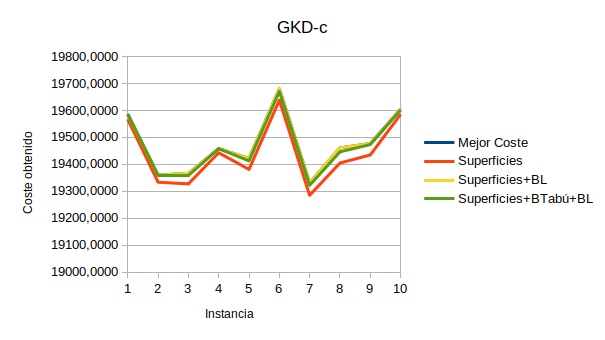
\includegraphics[scale=0.55]{img/aa.png}
\end{figure}

\item \texttt{MDG-a}: Conjunto de datos correspondiente al grupo de distancias enteras y tamaño de $n=2000$ y $m=200$. 
	\begin{figure}[H]
	\centering
	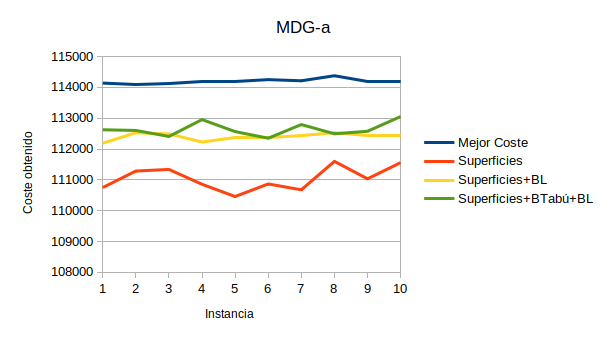
\includegraphics[scale=0.55]{img/c.png}
\end{figure}

	Se observa claramente que el perfil rojo referente a la versión original (sin hibridar) se encuentra por debajo de las otras dos implementaciones. Esto no quiere decir que dicho algoritmo sea malo, de hecho, mejora a todos los algoritmos genéticos de la práctica 2. 
	
	En relación con las versiones hibridadas (perfil amarillo y verde), vemos que en todas las instancias menos en 3 de ellas, hibridar el algoritmo con $BL$ y \textit{Búsqueda Tabú} mejora en gran medida. Esto era de esperar ya que a la hora de crear las distintas soluciones aleatorias, se han añadido algunas de 'calidad' por lo que no dependemos tanto de la aleatoriedad inicial de las soluciones.
	
	

 	\item \texttt{MDG-b}: Conjunto de datos correspondiente al grupo de distancias reales y tamaño $n=500$ y $m=50$. 
	\begin{figure}[H]
	\centering
	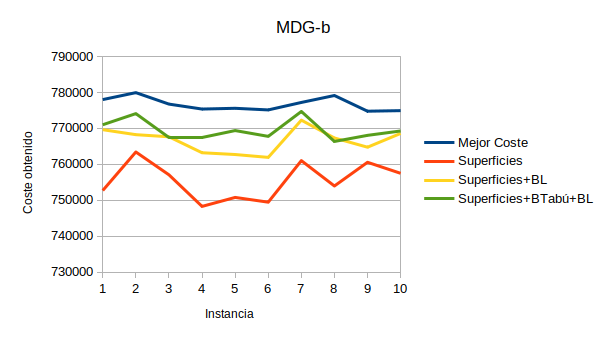
\includegraphics[scale=0.55]{img/b.png}
\end{figure}


\end{itemize}

	Destacamos los siguientes aspectos: 
	\begin{itemize}
		\item Al igual que ocurre en el grupo de instancias anterior, ambas versiones hibridadas mejoran bastante respecto al algoritmo original debido en cierto modo a las técnicas introducidas para evitar óptimos locales. 
		
		\item En relación con las versiones hibridadas, el claro ganador vuelve a ser la versión de \textit{Búsqueda Tabú + BL}
	\end{itemize}

 
 
 
 

\newpage


\subsection{Resultados de todos los algoritmos estudiados }

Mostramos a continuación un tabla a modo de resumen general de todos los algoritmos programados en la asignatura, separándolos en práctica 1, 2, 3 y proyecto final de teoría:



\[
\begin{array}{r|*{4}{r}}{Algoritmo}&Desv&Tiempo\\\hline


{}Greedy&1,37&0,46\\

{}BL&1,07&0.49\\
\hline 

{}AGG-posici$\'o$n&2,34&205,13\\

{}AGG-uniforme&2,53&190,37\\

{}AGE-posici$\'o$n&2,07&109,06\\

{}AGE-uniforme&1,42&315,41\\

{}AM-(10,1.0)&0,74&8,05\\

{}AM-(10,0.1)&0,89&65,92\\

{}AM-(10,1.0mej)&0,74&59,24\\

\hline 

{}ES&1,15&0,17\\

{}BMB&0,72&0,24\\

{}ILS&0,55&0,16\\

{}ILS\text{-}ES&0,70&1,78 \\

\hline 

{}Superficies&1,89&309,14\\

{}Superficies+BL&0,96&39,38\\

{}Superficies+B.Tab$\'u$ + BL&0,77&289,34

\end{array}
\label{glob}
\]

Como podemos comprobar, los resultados obtenidos en nuestros algoritmos de la entrega final  de teoría son bastante prometedores. Si se tuviera que destacar un algoritmo en especial, sería la \textit{Búsqueda Local} y todas sus versiones hibridadas.


\begin{itemize}
	\item En comparación con los algoritmos genéticos, vemos que la versión \textit{Superficies} (sin hibridar) mejora a todos los algoritmos genéticos a excepción del Algoritmo Genético Estacionario ($AGE$) en su versión uniforme.
	
	\item Sin embargo, en la versión hibridada con \textit{Búsqueda Local}, vemos que tanto los algoritmos meméticos como los programados en esta entrega muestran unas desviación muy parecida.
	
	\item Los mejores resultados se han obtenido en la práctica 3, tanto en eficacia como en eficiencia, en concreto \textit{Búsqueda Local Reiterada} ($ILS$), que como bien se comentó se trata de un algoritmo basado en trayectorias múltiples que usa el criterio del mejor como aceptación.
\end{itemize}

\newpage 
\section{Análisis de escalado}

Como bien se ha comentado en el punto anterior, los algoritmos híbridos con $BL$ muestran un comportamiento general y no podemos establecer un claro ganador ya que la diferencia de desviación entre unos algoritmos y otros es  muy baja.

Para todas estas ejecuciones, el criterio de parada era común, alcanzar 100.000 evaluaciones de la función objetivo. Por ello, realizamos una nueva ejecución de \textit{(AM-(10,1.0)), ILS y Superficies+BTabú+BL} pero estableciendo el criterio de parada a 400.000 evaluaciones.

Mostramos una tabla a modo de resumen de los resultados obtenidos (El estudio con todos las ejecuciones de las instancias se puede ver en el archivo \textit{Estudio.ods}, situado en la carpeta \textit{resultados}):




\[
\begin{array}{c|c|c}{Algoritmo}&Desv, 100k \hspace{0.1cm} eval & Desv, 400k \hspace{0.1cm} eval\\\hline

{}AM-(10,1.0)&0,74&0,60\\

{}ILS&0.55&0,54\\

{}Superficies+B.Tab$\'u$ + BL&0.77&0.46


\end{array}
\label{escalado}
\]




\hfill \break

Observando la tabla anterior y, para nuestro asombro, vemos que tras 400.000 evaluaciones, el  algoritmo \textit{Superficies} es el que mejores resultados obtiene, superando incluso al \textit{Algoritmo Memético} y  \textit{Búsqueda Local Reiterada} de las prácticas 2 y 3, respectivamente.

	\begin{figure}[H]
	\centering
	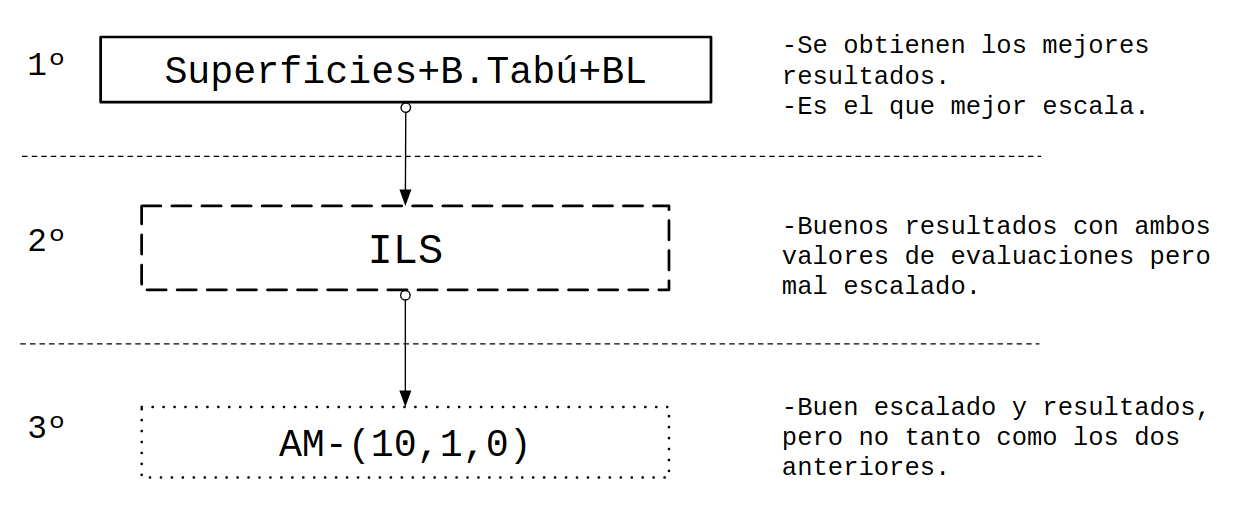
\includegraphics[scale=0.33]{img/final.png}
\end{figure}







\newpage 
\section{Futuros escenarios}

El conjunto inicial de superficies en nuestra implementación es de únicamente 4 y, a pesar de ello, los resultados obtenidos son bastante prometedores.

Se podría tomar un mayor número de superficies combinadas con el modelo distribuido en forma de isla, así, el número de entornos explorados serían aún mayor. Éstas superficies podrían además formarse a partir de sumas conexas (uniones) de las superficies anteriores. Destacamos lo siguiente:

\begin{itemize}
	\item La suma conexa de k-planos proyectivos será una superficie orientable mientras que la suma conexa de k-toros será orientable.
	
	En la siguiente imagen podemos ver la representación de un 2-toro que podemos perfectamente utilizar como superficie para nuestra propuesta.
	
	\begin{figure}[H]
	\centering
	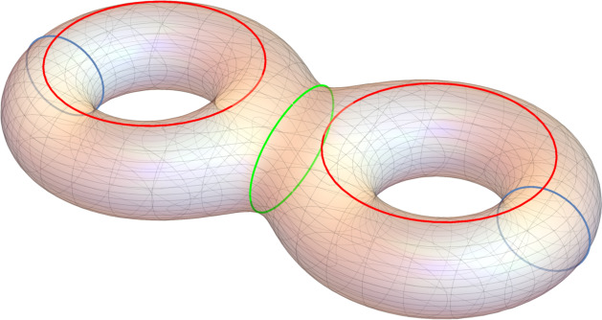
\includegraphics[scale=0.35]{img/2t.png}
	\end{figure}

	Sin embargo... ¿Cómo podemos llevar la representación de este 2-toro de forma rápida y sencilla a un tablero? 


	\item Para contestar a la pregunta anterior,  se ha realizado un programa adicional para simular el movimiento de una solución en un 2-toro y así ver cómo se comportarían las identificaciones en esta supercicie. Éste código se ha entregado junto al proyecto en 2 versiones, una en terminal y otra con interfaz gráfica, en el directorio \textit{snake/}
	
	
		\begin{figure}[H]
		\centering
		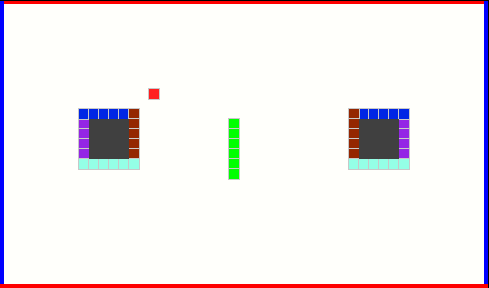
\includegraphics[scale=0.45]{img/yesh.png}
		\caption{snake/snake2-toro.gif}
	\end{figure}
	

\end{itemize}




A simple vista, podemos pensar que ambas figuras no son iguales ya que no se conservan las distancias (el recorrido por los arcos grises y rojos de la figura superior son distintos, mientras que esta distancia en la figura inferior no se tiene en cuenta), es decir, ambas figuras no tienen las misma geometría.
Sin embargo, topológicamente podemos afirmar que son equivalentes ya que mediante deformaciones podemos obtener una a partir de la otra.

Observando la última figura, vemos que en total tenemos 6 identificaciones luego nuestra solución está caracterizada por tener un entorno en el que 6 caracteres se mutarán, pero... ¿Tener un entorno con mayor número de mutaciones supondría unos mejores resultados?






\newpage
\begin{thebibliography}{X} 
	
-\href{https://sci2s.ugr.es/sites/default/files/files/Teaching/GraduatesCourses/Metaheuristicas/Sem01-Problemas-MHs-2019-20.pdf}{Seminario 1}\\
	
	-\href{https://sci2s.ugr.es/sites/default/files/files/Teaching/GraduatesCourses/Metaheuristicas/Sem02-Problemas-BusquedaLocal-MHs-19-20.pdf}{Seminario 2}\\
	
		-\href{https://sci2s.ugr.es/sites/default/files/Sem03-Problemas-Poblaciones-MHs-19-20.pdf}{Seminario 3}\\
		
		-\href{https://sci2s.ugr.es/sites/default/files/files/Teaching/GraduatesCourses/Metaheuristicas/Sem04-Problemas-Trayectorias-MHs-19-20.pdf}{Seminario 4}\\
	
	-\href{https://sci2s.ugr.es/sites/default/files/files/Teaching/GraduatesCourses/Metaheuristicas/MHs\%20-\%20Pr\%C3\%A1ctica-4-Para-evaluaci\%C3\%B3n-teoria-Junio-2020.pdf}{Práctica para evaluar teoría}




\end{thebibliography}


\end{document}

